\documentclass[a4paper]{article}
\usepackage{amsmath}
\usepackage{graphicx}
\usepackage{geometry}
\usepackage{floatrow}
\usepackage{layout}
\usepackage{amssymb} 
\usepackage{multirow}
\usepackage{caption}
\geometry{margin=1in}
\usepackage{authblk}
\usepackage{indentfirst}
\usepackage[hidelinks]{hyperref}
\usepackage{enumitem}
\usepackage{float}
\usepackage{hyperref}
\usepackage{amssymb}
\usepackage{xcolor}


\providecommand{\keywords}[1]
{
  \small	
  \textbf{\; \textit{Keywords---}} #1
}

\begin{document}

\title{\textbf{\huge{Problem Set 1}}}

\author{\textbf\large{Teera Tesharojanasup}}

\affil{\textbf{Northeastern University, Boston}}

\date{\text{July 10th, 2024}}

\maketitle
\begin{sloppypar}

\section*{Overview}

Problem set 1 for CS 4100 Summer II. Taught by assistant teaching professor, \href{https://rajagopalvenkat.com/}{Rajagopal Venkat}. \cite{MISC:1}

\section{Categorizing AI Environments}

\begin{enumerate}[start=1,label=Q\arabic*,left=0pt]
    \item \textbf{Under what (implementation-related) assumptions is maze-solving a fully observable environment? What are the agent’s percepts?}
    \par We would assume that the agent is able to have all the information regarding the maze environment to be able to determine if the maze
    is fully observable. 
    This would include the complete maze layout like the ways it can traverse, the walls, the starting position, and the exit position.
    Therefore, the agent's percept would be:
    \begin{itemize}
        \item The complete map of the maze.
        \item The agent's current location.
        \item The goal/exit location.
        \item The possible turns/moves it could make from its current position.
    \end{itemize}
    
    \item \textbf{Under what (implementation-related) assumptions is maze-solving a partially observable environment? What are the agent’s percepts?}
    \par A maze is partially observable if the agent has limited information. This would mean that the agent
    will not have all the information regarding the maze like all the walls and the ways it can traverse. Therefore,
    the agent's percept would be:
    \begin{itemize}
        \item An incomplete map of the maze (created when the agent moves around the maze).
        \item The agent's current location.
        \item The agent may only have limited information about the goal location like its general direction but not its exact coordinate.
        \item The agent can only sense/see the maze in its immediate surrounding.
    \end{itemize}
    
    \item \textbf{Is a known environment always fully observable? Explain with an example.}
    \par No, consider the game of solitaire. The agent knows the rules of this environment where in this case would be the rules
    of the card game making it a known environment. However, it is only partially observable since the agent will not know which card will
    appear next because this information is hidden.
    
    \item \textbf{Is a partially observable environment always an unknown environment? Explain with an example.}
    \par No, consider an agent that delivers coffee within Google's headquarter. The agent has general information about the office building,
    like the number of floors, elevator locations etc. This environment is only partially observable because the agent has limited visibility due to
    its visual, and auditory sensors. 
    
    However, this is not an unknown environment since the agent has an understanding of the building layout and
    can navigate its way to a location following certain sets of rules such as not bumping into employees, moving on certain designated office highways,
    utilizing elevators to move up/down floors etc.

    \item \textbf{What is the difference between an unknown environment and a non-deterministic environment? Explain with an example.}
    \par An unknown environment is one where we do not know the rules. In a non-deterministic environment, there is the factor of randomness/uncertainty. A good example
    of this is to visualize a drone visiting an unexplored alien planet with the goal of finding life. This is an unknown environment since we do not have any prior maps or information 
    about this planet. 
    
    It is also non-deterministic because the chances of discovering life is not certain. The creation of life is complicated,
    and although we do know what creates life, we cannot say for certainty that just because building blocks of life exists, that life will exist.

\end{enumerate}

\section{Search}

\par In this problem set, we will be using Rook Jumping Mazes (RJMs) - a game based on
Rook moves in Chess - to understand various search techniques. In a RJM, you are
given a square $n \times n$ grid, with each cell containing a number between $1$ to $n - 1$. From
any cell, the player may move either horizontally or vertically but must take exactly the
number of steps as shown on the player’s current cell. Regardless of the length of the
jump (i.e. number of cells passed), this action is considered a single jump (i.e., having a
cost of 1) for purposes of our search. The objective is to get from an assigned start state
to a pre-specified goal state. Consider this example:

\begin{figure}[H]
    \centering  
    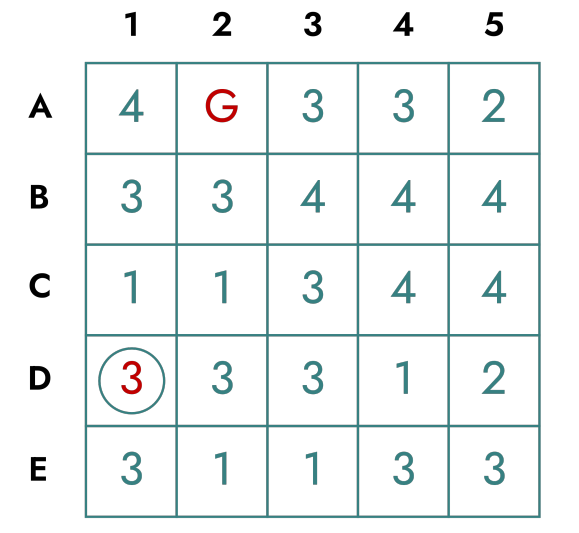
\includegraphics[height=0.2\textheight]{Search_RJM.png}
    \label{fig:Search_RJM}
\end{figure}

\noindent The cell D1 is the start state and the cell A2 is the goal state. The shortest solution to this
RJM is: [D1, A1, A5, C5, C1, C2, D2, A2]. Such a game lends itself well to the various
search algorithms we covered in class.

\begin{enumerate}[start=6,label=Q\arabic*,left=0pt]
    \item \textbf{Can both Breadth-First Search (BFS) and Depth-First Search (DFS) be used to solve RJMs? Will both yield the shortest path?}
    \par Yes, BFS and DFS can be used to solve RJMs. This is because we can turn a RJM into an unweighted graph which BFS and DFS 
    can be used for. 
    
    Breadth-First Search will find the shortest path because it searches all the surrounding nodes in the same level. Thus, BFS
    will be able to go down multiple branches and compare them allowing us to find the shortest path. However, DFS may not 
    always find the shortest path depending on which branch DFS chooses.

    \item \textbf{Assuming that each jump has a cost of 1, irrespective of the number of cells the rook
    passes while making that jump, we can use A* search to find the shortest path. Recall
    from class that A* search requires a consistent heuristic to guarantee an optimal solution.
    Show that for this problem, the Manhattan distance from any cell to the goal cell divided
    by (n - 1) is a consistent heuristic, where n is the number of cells in a row/column. In other words, show that}

    \[ H(node, goal, n) = \frac{|node_x - goal_x| + |node_y - goal_y|}{n - 1} \]

    \textbf{is a consistent heuristic. Remember that a proof may not rely on a single example, but instead must hold true in general.}
    
    \par Here, we want to proof that using the Manhattan distance, this equation holds true for all cases:
    \[ h(n) \leq c(n \rightarrow n') + h(n') \]
    Where $n = current\:node$ and $n' = neighbors\:of\:node\:n$. Starting at node n, we can move right, up, left or down:
    \begin{enumerate}[start=1,label=\arabic*.,left=0pt]
        \item $ x = k, \quad y = 0 $
        \item $ x = 0, \quad y = k $ 
        \item $ x = -k, \quad y = 0 $
        \item $ x = 0, \quad y = -k $
    \end{enumerate}

    Where $ k \in \{1, \ldots, n-1\} $.

    Case 1:
    \begin{align*}
        &\frac{|node_x - goal_x| + |node_y - goal_y|}{n - 1} \leq 1 + \frac{|(node_x + k) - goal_x| + |node_y - goal_y|}{n - 1} \\
        &\frac{|node_x - goal_x| + |node_y - goal_y|}{n - 1} - \frac{|(node_x + k) - goal_x| + |node_y - goal_y|}{n - 1} \leq 1 \\
        &\frac{|node_x - goal_x| - |(node_x + k) - goal_x|}{n - 1} \leq 1 \\
        &|node_x - goal_x| - |(node_x + k) - goal_x| \leq n - 1 \\\\
        &\text{Let} \:\: node_x - goal_x = f \\\\
        &|f| - |f + k| \leq n - 1 \\
        &-k \leq n - 1 \\
        &k \geq -n + 1 \\\\
        &\text{Lower End of k = 1} \\
        &1 \geq -n + 1 \\
        &n \geq 0 \\\\
        &\text{Upper End of k = n - 1} \\
        &n - 1 \geq -n + 1 \\
        &2n \geq 2 \\
        &n \geq 1 \\\\
        &\text{These inequalities will always hold true since n will always be at least 1.}
    \end{align*}

    Case 2:
    \begin{align*}
        &\frac{|node_x - goal_x| + |node_y - goal_y|}{n - 1} \leq 1 + \frac{|node_x - goal_x| + |(node_y + k) - goal_y|}{n - 1} \\
        &\frac{|node_x - goal_x| + |node_y - goal_y|}{n - 1} - \frac{|node_x - goal_x| + |(node_y + k) - goal_y|}{n - 1} \leq 1 \\
        &\frac{|node_y - goal_y| - |(node_y + k) - goal_y|}{n - 1} \leq 1 \\
        &|node_y - goal_y| - |(node_y + k) - goal_y| \leq n - 1 \\\\
        &\text{Let} \:\: node_y - goal_y = f \\\\
        &|f| - |f + k| \leq n - 1 \\
        &-k \leq n - 1 \\
        &k \geq -n + 1 \\\\
        &\text{Lower End of k = 1} \\
        &1 \geq -n + 1 \\
        &n \geq 0 \\\\
        &\text{Upper End of k = n - 1} \\
        &n - 1 \geq -n + 1 \\
        &2n \geq 2 \\
        &n \geq 1 \\\\
        &\text{These inequalities will always hold true since n will always be at least 1.}
    \end{align*}

    Case 3:
    \begin{align*}
        &\frac{|node_x - goal_x| + |node_y - goal_y|}{n - 1} \leq 1 + \frac{|(node_x - k) - goal_x| + |node_y - goal_y|}{n - 1} \\
        &\frac{|node_x - goal_x| + |node_y - goal_y|}{n - 1} - \frac{|(node_x - k) - goal_x| + |node_y - goal_y|}{n - 1} \leq 1 \\
        &\frac{|node_x - goal_x| - |(node_x - k) - goal_x|}{n - 1} \leq 1 \\
        &|node_x - goal_x| - |(node_x - k) - goal_x| \leq n - 1 \\\\
        &\text{Let} \:\: node_x - goal_x = f \\\\
        &|f| - |f - k| \leq n - 1 \\
        &k \leq n - 1 \\\\
        &\text{We know that k = [1, n - 1]} \\
        &[1, \: n - 1] \leq n - 1 \\\\
        &\text{Thus, we know that the statement above will always hold true because} \: n \: \\
        &\text{will always be at least 1.}
    \end{align*} 

    Case 4:
    \begin{align*}
        &\frac{|node_x - goal_x| + |node_y - goal_y|}{n - 1} \leq 1 + \frac{|node_x - goal_x| + |(node_y - k) - goal_y|}{n - 1} \\
        &\frac{|node_x - goal_x| + |node_y - goal_y|}{n - 1} - \frac{|node_x - goal_x| + |(node_y - k) - goal_y|}{n - 1} \leq 1 \\
        &\frac{|node_y - goal_y| - |(node_y - k) - goal_y|}{n - 1} \leq 1 \\
        &|node_y - goal_y| - |(node_y - k) - goal_y| \leq n - 1 \\\\
        &\text{Let} \:\: node_y - goal_y = f \\\\
        &|f| - |f - k| \leq n - 1 \\
        &k \leq n - 1 \\\\
        &\text{We know that k = [1, n - 1]} \\
        &[1, \: n - 1] \leq n - 1 \\\\
        &\text{Thus, we know that the statement above will always hold true because} \: n \: \\
        &\text{will always be at least 1.}
    \end{align*} 

    $\therefore \text{By proving all 4 cases, we can say that } H(node, goal, n) = \frac{|node_x - goal_x| + |node_y - goal_y|}{n - 1}$ \\ 
    $\text{is a consistent heuristic.} \hfill \blacksquare$
    
    \item \textbf{Consider the following RJM:}
    \begin{figure}[H]
        \centering  
        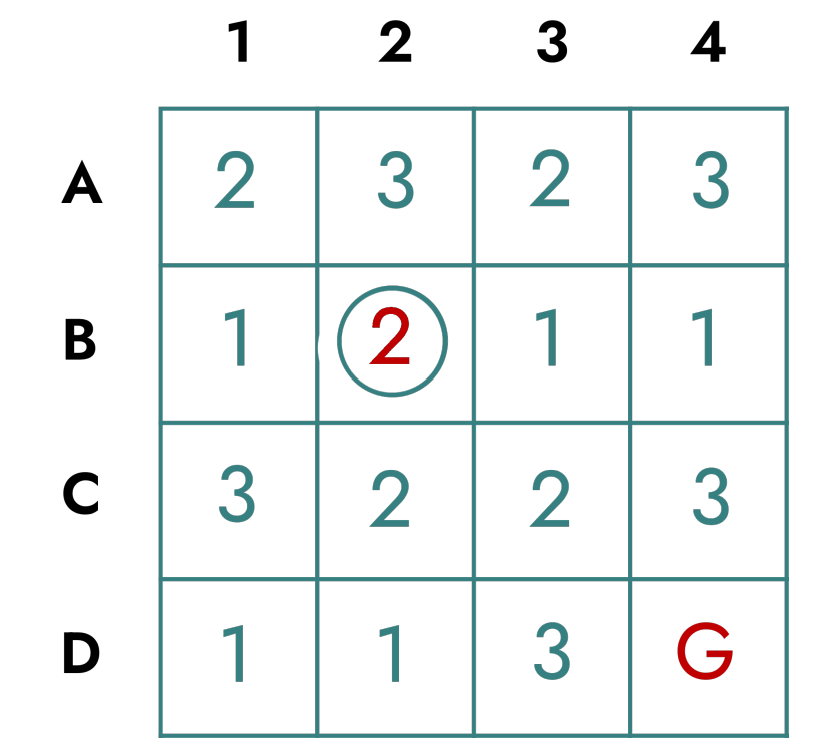
\includegraphics[height=0.2\textheight]{Q8_RJM.png}
        \label{fig:Q8_RJM}
    \end{figure}
    \textbf{On this maze, using the heuristic from Q7, complete the A* search process shown be- low, starting with Step 2. Terminate your search when the Goal node (cell D4) is popped from the priority queue. Double check your calculations!}
    
    \par Initialization:
    \begin{align*}\
        &\rightarrow \text{Starting at node B2} \\
        &B2 \: \text{Priority} = \text{cost} + H(B2) = 0 + \frac{4}{3} = \frac{4}{3} \\\\
        &\text{B2 Cost = 0} \\
        &\rightarrow \text{Push B2 to PQ} \\\\
        &\text{PQ} = \left\{\begin{array}{l}
            (v=B2, priority=\frac{4}{3}, cost=0, path=[])
        \end{array}\right\}
    \end{align*}

    \par Step 1:
    \begin{align*}
        &\rightarrow \text{Pop B2} \\
        &\text{Neighbor(s) of B2 = D2, B4} \\\\
        &D2 \: \text{Priority} = \text{cost} + \text{wt(B2, D2)} + H(D2) = 0 + 1 + \frac{2}{3} = \frac{5}{3} \\
        &B4 \: \text{Priority} = \text{cost} + \text{wt(B2, C4)} + H(B4) = 0 + 1 + \frac{2}{3} = \frac{5}{3} \\\\
        &\text{D2 Cost = 1, B4 cost = 1} \\
        &\rightarrow \text{Push D2, B4 to PQ} \\\\
        &\text{PQ} = \left\{\begin{array}{l}
            (v=D2, priority=\frac{5}{3}, cost=1, path=[B2]), \\
            (v=B4, priority=\frac{5}{3}, cost=1, path=[B2])
        \end{array}\right\}
    \end{align*}

    \par Step 2:
    \begin{align*}
        &\rightarrow \text{Pop D2} \\
        &\text{Neighbor(s) of D2 = D1, C2, D3} \\\\
        &D1 \: \text{Priority} = \text{cost} + \text{wt(D2, D1)} + H(D1) = 1 + 1 + 1 = 3 \\
        &C2 \: \text{Priority} = \text{cost} + \text{wt(D2, C2)} + H(C2) = 1 + 1 + 1 = 3 \\
        &D3 \: \text{Priority} = \text{cost} + \text{wt(D2, D3)} + H(D3) = 1 + 1 + \frac{1}{3} = \frac{7}{3} \\\\
        &\text{D1 Cost = 2, C2 cost = 2, D3 cost = 2} \\
        &\rightarrow \text{Push D1, C2, D3 to PQ} \\\\
        &\text{PQ} = \left\{\begin{array}{l}
            (v=B4, priority=\frac{5}{3}, cost=1, path=[B2]), \\
            (v=D3, priority=\frac{7}{3}, cost=2, path=[B2, D2]), \\
            (v=D1, priority=3, cost=2, path=[B2, D2]), \\
            (v=C2, priority=3, cost=2, path=[B2, D2])
        \end{array}\right\}
    \end{align*}

    \par Step 3:
    \begin{align*}
        &\rightarrow \text{Pop B4} \\
        &\text{Neighbor(s) of B4 = A4, B3, C4} \\\\
        &A4 \: \text{Priority} = \text{cost} + \text{wt(B4, A4)} + H(A4) = 1 + 1 + 1 = 3 \\
        &B3 \: \text{Priority} = \text{cost} + \text{wt(B4, B3)} + H(B3) = 1 + 1 + 1 = 3 \\
        &C4 \: \text{Priority} = \text{cost} + \text{wt(B4, C4)} + H(C4) = 1 + 1 + \frac{1}{3} = \frac{7}{3} \\\\
        &\text{A4 Cost = 2, B3 cost = 2, C4 cost = 2} \\
        &\rightarrow \text{Push A4, B3, C4 to PQ} \\\\
        &\text{PQ} = \left\{\begin{array}{l}
            (v=D3, priority=\frac{7}{3}, cost=2, path=[B2, D2]), \\
            (v=C4, priority=\frac{7}{3}, cost=2, path=[B2, B4]), \\
            (v=A4, priority=3, cost=2, path=[B2, B4]), \\
            (v=C2, priority=3, cost=2, path=[B2, D2]), \\
            (v=D1, priority=3, cost=2, path=[B2, D2]), \\
            (v=B3, priority=3, cost=2, path=[B2, B4])
        \end{array}\right\}
    \end{align*}

    \par Step 4:
    \begin{align*}
        &\rightarrow \text{Pop D3} \\
        &\text{Neighbor(s) of D3 = A3} \\\\
        &A3 \: \text{Priority} = \text{cost} + \text{wt(D3, A3)} + H(A3) = 2 + 1 + \frac{4}{3} = \frac{13}{3} \\\\
        &\text{A3 Cost = 3} \\
        &\rightarrow \text{Push A3 to PQ} \\\\
        &\text{PQ} = \left\{\begin{array}{l}
            (v=C4, priority=\frac{7}{3}, cost=2, path=[B2, B4]), \\
            (v=A4, priority=3, cost=2, path=[B2, B4]), \\
            (v=C2, priority=3, cost=2, path=[B2, D2]), \\
            (v=D1, priority=3, cost=2, path=[B2, D2]), \\
            (v=B3, priority=3, cost=2, path=[B2, B4]), \\
            (v=A3, priority=\frac{13}{3}, cost=3, path=[B2, D2, D3])
        \end{array}\right\}
    \end{align*}

    \par Step 5:
    \begin{align*}
        &\rightarrow \text{Pop C4} \\
        &\text{Neighbor(s) of C4 = C1} \\\\
        &C1 \: \text{Priority} = \text{cost} + \text{wt(C4, C1)} + H(C1) = 2 + 1 + \frac{4}{3} = \frac{13}{3} \\\\
        &\text{C1 Cost = 3} \\
        &\rightarrow \text{Push C1 to PQ} \\\\
        &\text{PQ} = \left\{\begin{array}{l}
            (v=A4, priority=3, cost=2, path=[B2, B4]), \\
            (v=C2, priority=3, cost=2, path=[B2, D2]), \\
            (v=D1, priority=3, cost=2, path=[B2, D2]), \\
            (v=B3, priority=3, cost=2, path=[B2, B4]), \\
            (v=A3, priority=\frac{13}{3}, cost=3, path=[B2, D2, D3]), \\
            (v=C1, priority=\frac{13}{3}, cost=3, path=[B2, B4, C4])
        \end{array}\right\}
    \end{align*}

    \par Step 6:
    \begin{align*}
        &\rightarrow \text{Pop A4} \\
        &\text{Neighbor(s) of A4 = A1, D4} \\\\
        &A1 \: \text{Priority} = \text{cost} + \text{wt(A4, A1)} + H(A1) = 2 + 1 + 2 = 5 \\
        &D4 \: \text{Priority} = \text{cost} + \text{wt(A4, D4)} + H(D4) = 2 + 1 + 0 = 3 \\\\
        &\text{A1 Cost = 3, D4 Cost = 3} \\
        &\rightarrow \text{Push A1, D4 to PQ} \\\\
        &\text{PQ} = \left\{\begin{array}{l}
            (v=D4, priority=3, cost=3, path=[B2, B4, A4]) \\
            (v=C2, priority=3, cost=2, path=[B2, D2]), \\
            (v=D1, priority=3, cost=2, path=[B2, D2]), \\
            (v=B3, priority=3, cost=2, path=[B2, B4]), \\
            (v=A3, priority=\frac{13}{3}, cost=3, path=[B2, D2, D3]), \\
            (v=C1, priority=\frac{13}{3}, cost=3, path=[B2, B4, C4]), \\
            (v=A1, priority=5, cost=3, path=[B2, B4, A4])
        \end{array}\right\}
    \end{align*}

    \par Step 7:
    \begin{align*}
        &\rightarrow \text{Pop D4} \quad (v=D4, priority=3, cost=3, path=[B2, B4, A4]) \\
        &\rightarrow \text{Goal is found!} \\
        &\rightarrow \text{Append v = D4 to path} \\
        &\rightarrow \text{return path = [B2, B4, A4, D4]} \\
        &\textcolor{red}{\textbf{Terminate Program}}
    \end{align*}

\end{enumerate}

\section{Local Search}

Your professor is a coffee snob, and since he knows a thing or two about AI, he tries to
build an espresso machine that will learn a user’s preferences over time to pull the perfect
shot. He lets the machine control the following values:

\begin{itemize}
    \item Weight of coffee beans (15-21 grams)
    \item Grind size (250 - 400 microns)
    \item Water Pressure (7 - 11 bars)
    \item Brew time (27 - 33 seconds)
\end{itemize}

\begin{enumerate}[start=9,label=Q\arabic*,left=0pt]
    \item \textbf{Based on our discussions in class, is this problem well-suited to local search algorithms? Explain your reasoning.}
    \par This problem aims to learn the user’s preferences to create the most optimal coffee mix tailored to the user. 
    In other words, the focus is on the final solution rather than the specific optimizations or paths taken to achieve the perfect mix. 
    Conveniently, local search algorithms are designed for this type of problem, making them well-suited for finding the ideal solution.
    
    \item \textbf{How you would implement such a program? What would be a reasonable objective function? (This question is somewhat open-ended, so don’t worry too much about the ‘right’ answer. I am really looking for whether your thought process reflects a solid understanding of how local search works.)}
    \par I would use a hill-climbing algorithm. I would define the objective function to be based on user feedback.
    Lets say for each cup of coffee this machine brews, the user rates the coffee from 1 to 10 where 10 would mean perfect.
    The objection function $f(x)$ would try to maximize the user rating. However, if we want to use gradient descent, we can manipulate the 
    user rating by doing 
    
    \[f(x) = 10 - User Rating(x)\]

    This would mean that a user rating of 10 becomes:

    \[ f(x) = 10 - 10 = 0 \quad \xleftarrow{\text{best value}} \]

    and a user rating of 1 becomes:

    \[ f(x) = 10 - 1 = 9 \quad \xleftarrow{\text{worst value}} \]

    If we do this, we can frame the objective function from maximizing to minimizing $f(x)$ and thus perform gradient descent
    to find the optimal coffee blend.

    \item \textbf{Which of the optimizations and local search variants discussed in class (random restarts, varying step size, simulated annealing and genetic algorithms) are applicable to this problem, and why?}
    \par All 4 techniques are applicable to this solution. For random restarts, lets assume we are trying to minimize the objective
    function, the optimization algorithm we are using may get stuck inside a valley which may not be the global minimum. By using random
    restarts, we will be able to move to a different spot and hopefully find a better minimum.

    Varying step size can also be useful in finding the optimal solution. We can start with a larger step size to allow the algorithm
    to traverse a greater area of the search space and gradually reduce the step size as we hone in on a solution. 

    For simulated annealing, this technique accepts a worse solution with a probability that decreases over time. This encourages the algorithm
    to explore a larger area that surrounds the initial starting position in the hopes of finding a better local minimum and avoid being trapped
    inside a valley. 

    Lastly, genetic algorithms will allow the algorithm to explore multiple solutions that evolve/change over time. For example,
    it is common for a person's taste to change over time, and since genetic algorithms thrive based on the concept of change, it is particularly suited
    to this problem as it can adapt the espresso's machine mixture according to the user's changing tastes.
\end{enumerate}

\section{Adversarial Search}

\begin{enumerate}[start=12,label=Q\arabic*,left=0pt]
    \item \textbf{Construct a game tree example with a depth of 4 and a branching factor of 2, that illustrates the best-case for alpha-beta pruning, except for the trivial solution. Hand drawn figures accepted for this question, but please ensure clarity.}
    \begin{figure}[H]
        \centering  
        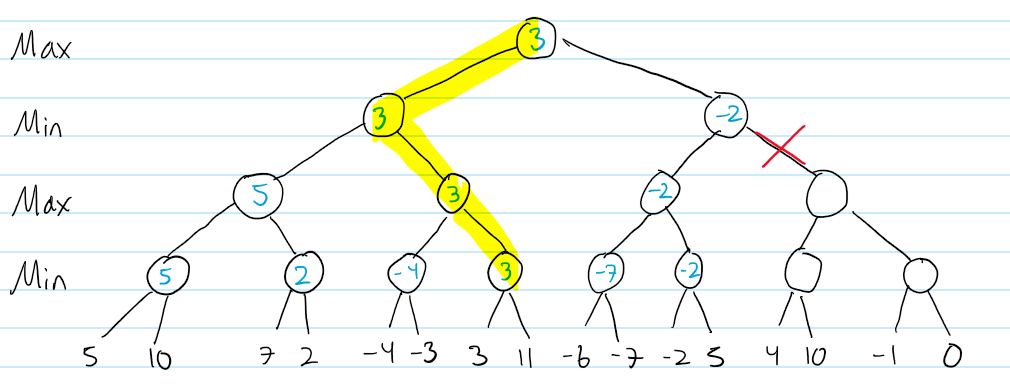
\includegraphics[height=0.2\textheight]{Q12_tree.png}
        \label{fig:Q12_tree}
    \end{figure}

    \item \textbf{Why is it desirable to combine iterative deepening with alpha-beta pruning from a practical standpoint?}
    \par Iterative deepening allows us to use DFS's low memory requirement combined with BFS's ability to explore multiple solutions.
    Alpha-beta pruning, on the other hand, reduces the number of nodes/branches needed to be evaluated and explored speeding up the search
    by eliminating branches that cannot influence the final decision.

    By combining these two together, the search can hone-in on more promising paths due to iterative deepening and
    skip exploring paths that are redundant. This will allow us to perform the search on a much bigger tree due to the low memory usage
    but at the same time, find a relatively good solution in a timely manner.

\end{enumerate}

\section{Academic Integrity}

\begin{enumerate}[start=14,label=Q\arabic*,left=0pt]
    \item \textbf{Review, and copy/paste the academic integrity acknowledgement in your final submission as the answer to Q14.}
    \par I have read and understood the academic integrity policy as outlined in the course syllabus for CS4100. 
    By pasting this acknowledgement in my submission, I declare that all work presented here is my own, 
    and any conceptual discussions I may have had with classmates have been fully disclosed. I declare that generative AI 
    was not used to answer any questions in this assignment. Any use of generative AI to improve writing clarity 
    alone is accompanied by an appendix with my original, unedited answers.
\end{enumerate}
\end{sloppypar}

\bibliography{references}
\bibliographystyle{ieeetr}

\end{document}